% begin module arc-length-derivation
\begin{frame}
\begin{itemize}
\item  What about $y = f(x)$ for a continuous function $f$ on $[a, b]$?
\item<2->  Divide $[a,b]$ into $n$ subintervals with endpoints $x_0, x_1, \ldots , x_n$ and equal width $\Delta x$.
\item<3->  The points $P_i = (x_i, f(x_i))$ lie on $y = f(x)$, and the segments with vertices $P_0, P_1, \ldots , P_n$ are an approximation to $y = f(x)$.
\item<4->  The length $L$ of the curve $y = f(x)$ is the limit of the lengths of these segments as $n\rightarrow \infty$.
\end{itemize}
\begin{columns}[c]
\column{.6\textwidth}
\begin{center}
\ \only<handout:0| -1>{%
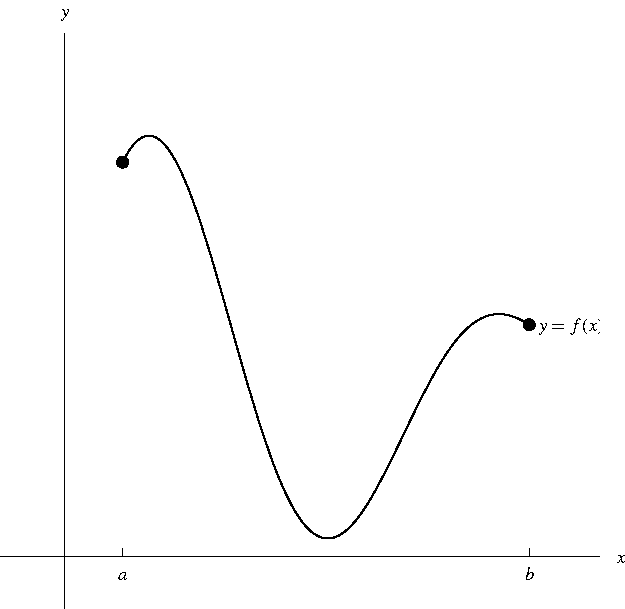
\includegraphics[height=4.5cm]{arc-length/pictures/09-01-arclengtha.pdf}%
}%
\only<handout:0| 2-4>{%
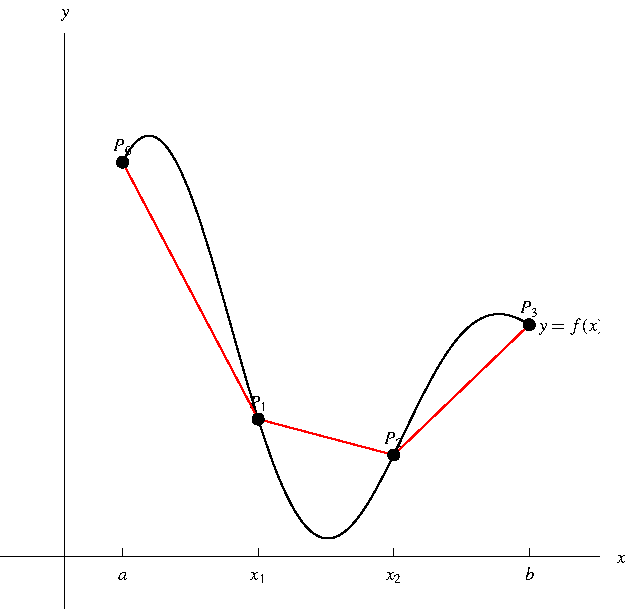
\includegraphics[height=4.5cm]{arc-length/pictures/09-01-arclengthb.pdf}%
}%
\only<handout:0| 5>{%
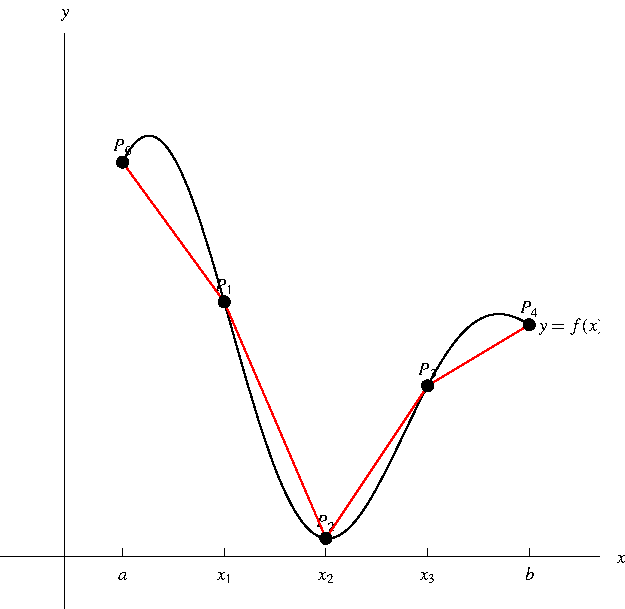
\includegraphics[height=4.5cm]{arc-length/pictures/09-01-arclengthc.pdf}%
}%
\only<handout:0| 6>{%
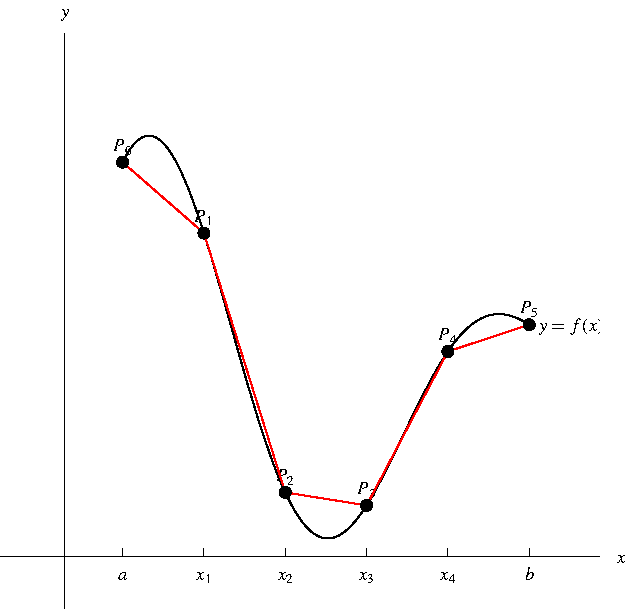
\includegraphics[height=4.5cm]{arc-length/pictures/09-01-arclengthd.pdf}%
}%
\only<handout:0| 7>{%
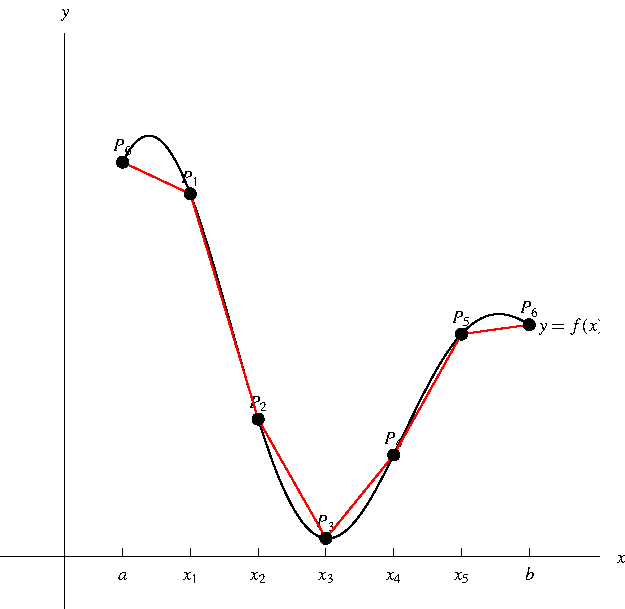
\includegraphics[height=4.5cm]{arc-length/pictures/09-01-arclengthe.pdf}%
}%
\only<8>{%
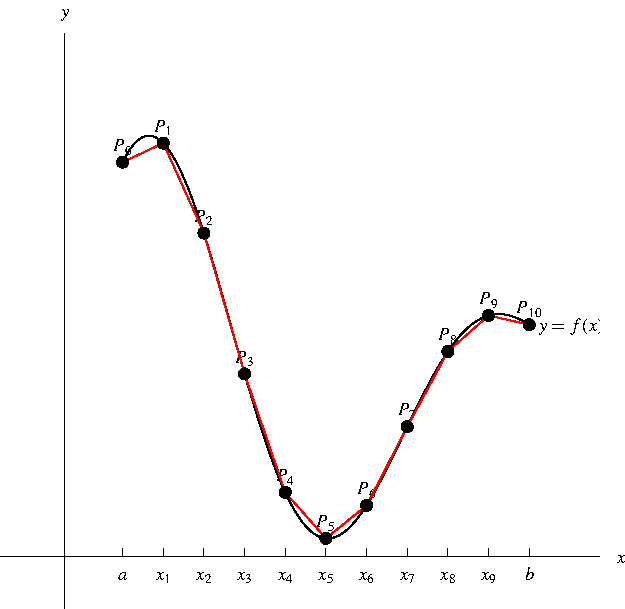
\includegraphics[height=4.5cm]{arc-length/pictures/09-01-arclengthf.pdf}%
}%
\only<handout:0| 9->{%
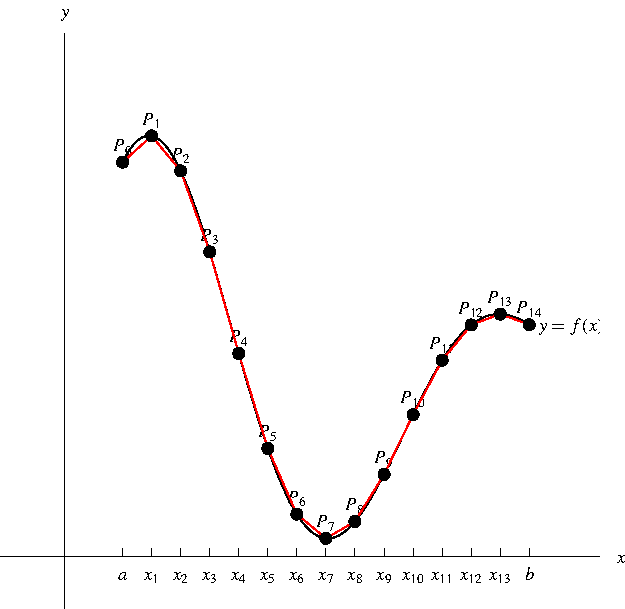
\includegraphics[height=4.5cm]{arc-length/pictures/09-01-arclengthg.pdf}%
}%
%\only<10->{%
%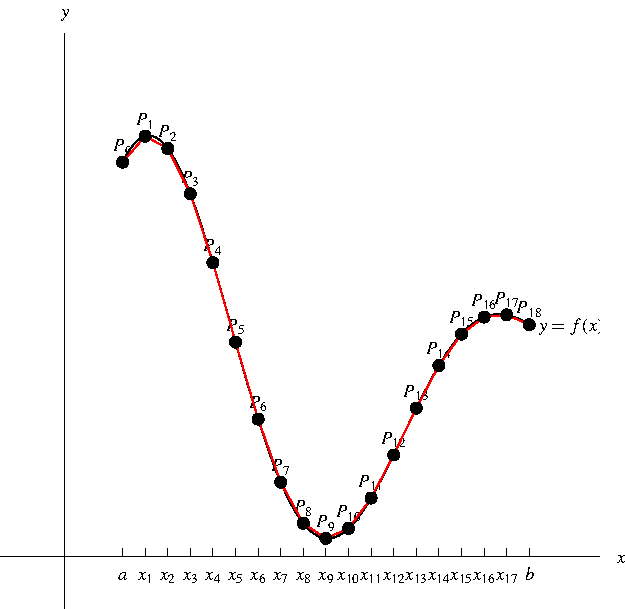
\includegraphics[height=4.5cm]{arc-length/pictures/09-01-arclengthh.pdf}%
%}%
\end{center}
\column{.4\textwidth}
\uncover<10->{%
\[
L = \lim_{n\rightarrow \infty} \sum_{i=1}^n |P_{i-1}P_i|
\]
}%
\end{columns}
\end{frame}



\begin{frame}
\begin{eqnarray*}
\uncover<1->{%
L = \lim_{n\rightarrow \infty} \sum_{i = 1}^n \alert<handout:0| 10>{|P_{i-1}P_i|}%
}%
& \uncover<10->{ = } &%
\uncover<10->{%
\alert<handout:0| 12>{\lim_{n\rightarrow\infty} \sum_{i=1}^n} \alert<handout:0| 10>{\sqrt{1+\alert<handout:0| 13>{(f'(x_i^*))^2}}\ \alert<handout:0| 14>{\Delta x}}%
}\\%
& \uncover<11->{ = } &%
\uncover<11->{%
\alert<handout:0| 12>{\int_a^b} \sqrt{1+\alert<handout:0| 13>{(f'(x))^2}} \ \alert<handout:0| 14>{\diff x}%
}%
\end{eqnarray*}
\begin{itemize}
\item  This formula is not useful for computational purposes.
\item  We can find a better formula when $f$ has a continuous derivative.
\item<2->  Let $y_i = f(x_i)$, and $\Delta y = y_i - y_{i-1} = f(x_i) - f(x_{i-1})$.
\item<3-| alert@6>  Then $|P_iP_{i-1}| = \sqrt{(x_i-x_{i-1})^2+(y_i-y_{i-1})^2} = \sqrt{(\Delta x)^2 + (\Delta y)^2}$.
\item<4->  Mean Value Theorem: there exists $x_i^*$ between $x_{i-1}$ and $x_i$ such that $\alert<handout:0| 5>{f(x_i) - f(x_{i-1}) = f'(x_i^*)(x_i-x_{i-1})}$.
\item<5-| alert@5,7>  $\Delta y = f'(x_i^*)\Delta x$.
\end{itemize}
\begin{eqnarray*}
\uncover<6->{%
\alert<handout:0| 10>{|P_{i-1}P_i|}%
}%
& \uncover<6->{\alert<handout:0| 10>{ = }} &%
\uncover<6->{%
\sqrt{(\Delta x)^2 + (\alert<handout:0| 7>{\Delta y})^2}%
}  \uncover<7->{ = } \uncover<7->{%
\sqrt{(\Delta x)^2 + (\alert<handout:0| 7>{f'(x_i^*)\Delta x})^2}%
}\\%
& \uncover<8->{ = } &%
\uncover<8->{%
\sqrt{1 + (f'(x_i^*))^2}\sqrt{(\Delta x)^2}%
}  \uncover<9->{ = } \uncover<9->{%
\alert<handout:0| 10>{\sqrt{1 + (f'(x_i^*))^2}\ \Delta x}%
}\\%
\end{eqnarray*}
\end{frame}
% end module arc-length-derivation
